\documentclass[journal]{IEEEtran}

% --- Packages ---
\usepackage{cite}
\usepackage{amsmath,amssymb,amsfonts}
\usepackage{algorithm}
\usepackage{algorithmic}
\usepackage{graphicx}
\usepackage{booktabs}
\usepackage{array}
\usepackage{multirow}
\usepackage{tabularx}
\usepackage{url}
\usepackage{xcolor}
\usepackage{balance}
\usepackage{placeins}
\usepackage{tikz}
\usepackage{pgfplots}
\usetikzlibrary{arrows.meta,positioning}
\pgfplotsset{compat=1.18}
\setlength{\textfloatsep}{11pt plus 2pt minus 2pt}
\setlength{\floatsep}{10pt plus 2pt minus 2pt}
\setlength{\intextsep}{10pt plus 2pt minus 2pt}
\setlength{\dbltextfloatsep}{11pt plus 2pt minus 2pt}

% --- Graphics Path ---
\graphicspath{{./}}

% --- Document Start ---
\begin{document}

\title{PeopleFlow: A Reproducible Geometry-Aware Multi-Agent Framework for Comparative Building Evacuation Safety Evaluation}

\author{Likith Sai Kunchi%
\thanks{Likith Sai Kunchi is with B.Tech CSE (SCOPE), VIT (Vellore Institute of Technology), India (e-mail: likithsai.kunchi@gmail.com).}}

\maketitle

\begin{abstract}
Evaluating evacuation performance in complex buildings requires analysis methods that capture the interaction between spatial configuration, pedestrian behavior, and operational disruptions. This paper introduces PeopleFlow, a geometry-informed computational framework designed to quantify evacuation effectiveness across diverse architectural layouts. The approach converts floor-plan representations into navigable simulation environments and applies continuous-space multi-agent modeling based on force-driven pedestrian dynamics. The system generates analytically meaningful indicators including total clearance duration, localized congestion intensity, persistence of bottleneck regions, and distribution balance across available exits.

To enable consistent experimentation, the framework incorporates parameterized scenario configurations and reproducibility-oriented execution records. The evaluation includes a structured matrix of nine layout types across five operational conditions, resulting in 450 core simulation runs, complemented by 90 additional controlled experiments examining real-layout generalization and parameter sensitivity involving exit width, walking-speed preference, and occupant scaling. Observed results indicate strong dependence of evacuation performance on geometric topology and routing strategy, with clearance duration differences exceeding an eightfold range and substantial variation in congestion intensity across layouts.

The primary contribution is a reproducible engineering evaluation framework enabling systematic relative safety prioritization across heterogeneous architectural configurations rather than deterministic prediction of individual trajectories. The proposed framework supports systematic what-if evaluation during early design stages and provides a computational basis for integration within digital twin environments for safety-oriented planning of high-occupancy infrastructure. The findings emphasize the importance of structured scenario evaluation to identify geometry-induced congestion risks and to support evidence-driven improvement of evacuation robustness.
\end{abstract}

\begin{IEEEkeywords}
Multi-agent simulation, evacuation modeling, crowd safety, building evacuation, digital twins, floor-plan analytics, safety engineering.
\end{IEEEkeywords}

\section{Introduction}
Building evacuation performance evaluation is a high-impact engineering task where static compliance checks often miss dynamic crowd effects under disruption. Historical emergencies consistently show that bottleneck formation, uneven exit utilization, and localized panic response can dominate outcomes even in code-compliant facilities. Conventional hand calculations remain useful for baseline checks, but they provide limited support for comparing design alternatives under multi-hazard and operational uncertainty \cite{sfpe,evac_review}.

Recent high-density infrastructure such as airports, metro systems, hospitals, and large commercial complexes introduces complex evacuation dynamics that cannot be fully evaluated using static compliance rules alone.

The need for early-stage design validation has increased with higher occupancy density in modern infrastructure. Although simulation enables repeatable structured comparison before deployment, the central challenge is integrating architectural input, scenario control, execution, and interpretable outputs within one coherent computational workflow.

The present research introduces PeopleFlow as a geometry-informed evacuation efficiency framework with traceable computational pipeline execution. Rather than proposing a new pedestrian-physics law in isolation, the study develops a unified computational workflow for robust scenario-based evaluation across heterogeneous layouts.

The three primary contributions are:
\begin{itemize}
    \item A reproducible floor-plan-aware evacuation evaluation workflow linking layout ingestion, scenario execution, and artifact-backed reporting.
    \item A multi-layout statistical comparison across 540 simulations (450 core + 90 supplementary) spanning diverse building archetypes.
    \item A density-aware routing evaluation under structured stress scenarios, supported by ablation and sensitivity analysis.
\end{itemize}

PeopleFlow is designed as a comparative decision-support workflow rather than an exact predictor of individual human trajectories.
Unlike prior evacuation simulation studies that primarily focus on behavioral model refinement, this work emphasizes workflow reproducibility, cross-layout comparability, and experiment-traceable safety evaluation.

\section{Related Work}
\subsection{Crowd Modeling Approaches}
Pedestrian evacuation research spans both continuous and discrete formulations. In force-based formulations, evacuees can be represented as self-driven particles whose motion evolves through interaction potentials capturing repulsion, attraction, and directional preference; this family remains a physically interpretable baseline for dense-crowd analysis \cite{sfm,helbing2000}. Cellular automata and floor-field variants offer efficient large-scale approximations but may introduce directional discretization artifacts near bottlenecks and tight corners \cite{ca,kirchner2002}. Comparative studies indicate that model suitability is task-dependent; for complex indoor geometries, continuous-space approaches often preserve turning behavior and local interaction structure more naturally \cite{zheng2009,duives2013,crowd_book}.

\subsection{Evacuation Simulation Systems}
Commercial and academic evacuation platforms generally cover geometry authoring, route simulation, and report generation, but they differ substantially in automation depth, extensibility, and experiment traceability \cite{path_planning,ronchi2015,lovreglio2020}. Behavior-focused studies further show that guidance logic, uncertainty handling, and panic-modulated decisions can materially alter evacuation outcomes \cite{pan2007,chen2018}. In many practical settings, heavy manual preprocessing and proprietary tooling still constrain transparent cross-layout benchmarking.

\subsection{Digital Twin Safety Analysis}
Digital twin studies in the built environment increasingly target safety and emergency operations. Prior work supports simulation-coupled twins for risk-aware planning, yet complete pipelines from floor-plan ingestion to repeatable quantitative evacuation indicators remain limited in many deployments \cite{sharma2020,chu2022,batty2012,zhang2021dtwins}. Recent building-fire twin systems also demonstrate practical monitoring and control integration for emergency analytics, reinforcing the need for end-to-end reproducible computational workflows \cite{ding2023jbe,jiang2023autcon}.

\subsection{Research Gap and Positioning}
The gap addressed in this paper is methodological: reproducible, geometry-informed evacuation efficiency comparison across diverse layouts and stress scenarios. PeopleFlow is positioned as a reproducible framework rather than a claim of absolute predictive certainty. Its novelty lies in coupling geometry extraction, session-managed simulation, scenario ablation, and interpretable reporting within one coherent computational workflow.
Unlike many existing evacuation simulators that require manual geometry preparation or proprietary workflows, PeopleFlow emphasizes reproducibility through artifact-backed records, enabling transparent cross-layout comparison under consistent scenario definitions.
A concise capability comparison with representative tools is provided in Table \ref{tab:tool_comparison}.

\begin{table}[t]
\centering
\caption{Comparison with Existing Evacuation Tools}
\label{tab:tool_comparison}
{\footnotesize
\setlength{\tabcolsep}{3pt}
\begin{tabular}{>{\bfseries}p{1.45cm} p{1.55cm} p{2.05cm} p{1.60cm}}
\toprule
Tool & Floor Plan Input & Routing & Reproducibility \\
\midrule
Pathfinder & Mostly manual & Shortest path / scripted & Limited \\
MassMotion & Mostly manual & Dynamic multi-agent & Proprietary workflow \\
AnyLogic & Complex model setup & Customizable & Moderate \\
Legion tools & Manual authoring & Flow-oriented & Limited \\
PeopleFlow & Automated ingestion & Congestion-aware & High (session-based) \\
\bottomrule
\end{tabular}
}
\end{table}

\section{Methodology}
\subsection{Workflow Pipeline}
PeopleFlow follows a deterministic workflow with four stages: (1) floor-plan ingestion, (2) geometry extraction and navigation graph generation, (3) scenario-based simulation execution, and (4) artifact-backed analytics. Each run is stored with configuration metadata, seeds, and per-step metrics so results are replayable and auditable. The step-level simulation procedure is summarized in Algorithm \ref{alg:simloop}.

\subsection{Reproducibility Design}
Each experiment is represented by a session artifact that captures:
\begin{itemize}
    \item Input layout identifier and geometry hash.
    \item Scenario parameters (occupancy, blocked exits, routing policy, panic level).
    \item Random seed and simulation step size.
    \item Aggregated outputs and raw trajectory summaries.
\end{itemize}
This structure allows direct reruns and supports batch-level statistical comparisons. The modular organization also enables independent evaluation of routing logic without modifying geometric preprocessing components. Simulation configurations and synthetic benchmark layouts are packaged as reproducible experiment artifacts and can be released to support future comparative studies. The implementation and reproducibility assets are maintained at \url{https://github.com/1206likith/PeopleFlow}.
A 30-second multimedia supplement demonstrating the end-to-end ingestion-to-analytics workflow is included in the submission artifacts.

\subsection{Agent Decision Logic}
At each simulation step, agents execute a compact perception-decision-motion loop. This structure ensures behavioral consistency while allowing routing-policy variation to be isolated during controlled ablation experiments. Local density and queue conditions are sensed first, then exit costs are updated using Eq. (\ref{eq:cost}). The lowest-cost exit is selected, social-force dynamics are integrated, and state variables are updated for the next step.

\begin{figure}[t]
\centering
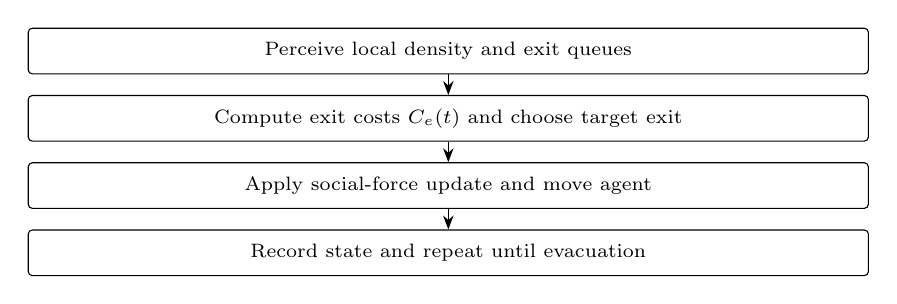
\begin{tikzpicture}[
    box/.style={draw, rounded corners=1.5pt, align=center, minimum width=0.88\columnwidth, minimum height=0.58cm, font=\scriptsize},
    arr/.style={-Stealth, line width=0.45pt}
]
\node[box] (s1) {Perceive local density and exit queues};
\node[box, below=2.6mm of s1] (s2) {Compute exit costs $C_e(t)$ and choose target exit};
\node[box, below=2.6mm of s2] (s3) {Apply social-force update and move agent};
\node[box, below=2.6mm of s3] (s4) {Record state and repeat until evacuation};
\draw[arr] (s1) -- (s2);
\draw[arr] (s2) -- (s3);
\draw[arr] (s3) -- (s4);
\end{tikzpicture}
\caption{Agent movement logic used in each simulation step.}
\label{fig:agent_logic}
\end{figure}

\subsection{Computational Complexity}
The computational complexity of a single simulation step is $O(Nk)$, where $N$ is the number of active agents and $k$ is the average number of neighboring agents considered in local interaction-force updates. Under practical density regimes, $k$ remains locally bounded, giving near-linear scaling with population size for each step. For batch execution, total workload scales as $O(RNS)$, where $R$ is the number of runs and $S$ is the number of simulation steps per run. This complexity profile motivates the reproducible batch workflow used in our large-matrix experiments.

\subsection{Scenario Matrix}
The study uses a five-scenario matrix reflecting realistic stress transitions from nominal operation to disruption. Table \ref{tab:scenarios} summarizes the definitions.

\begin{table}[t]
\centering
\caption{Scenario Definitions}
\label{tab:scenarios}
{\footnotesize
\setlength{\tabcolsep}{3pt}
\begin{tabular}{>{\bfseries}p{1.55cm} p{5.10cm}}
\toprule
Scenario & Description \\
\midrule
S1 Baseline & Nominal occupancy and shortest-path routing. \\
S2 HighOcc & Increased occupancy stress to test crowding sensitivity. \\
S3 Blocked & One major exit disabled to evaluate rerouting resilience. \\
S4 Routing & Congestion-aware routing policy activated. \\
S5 Panic & Stochastic panic variation in desired speed and interactions. \\
\bottomrule
\end{tabular}
}
\end{table}

\begin{algorithm}[t]
\caption{PeopleFlow Simulation Loop}
\label{alg:simloop}
\begin{algorithmic}[1]
\STATE \textbf{Input:} geometry $G$, scenario $S$, agents $N$, and step $\Delta t$
\STATE Initialize agents at valid non-overlapping spawn locations
\STATE Set routing and behavior parameters from $S$
\WHILE{not all agents evacuated and $t < T_{max}$}
    \FOR{each agent $i$}
        \STATE Evaluate target exit based on the active routing policy
        \STATE Compute driving, interaction, and wall forces
        \STATE Update velocity and position via forward integration
    \ENDFOR
    \STATE Update local density map and congestion indicators
    \STATE Record per-step metrics and event logs
    \STATE $t \leftarrow t + \Delta t$
\ENDWHILE
\STATE Aggregate run-level metrics and persist session artifacts
\end{algorithmic}
\end{algorithm}

\section{PeopleFlow Architecture}
\subsection{System Components}
The architecture consists of geometry ingestion, simulation kernel, metrics engine, and reporting layer. Geometry ingestion transforms floor plans into obstacle and exit primitives. The simulation kernel executes force-based motion and route updates. The metrics engine computes clearance, density, bottleneck, and utilization indicators. The reporting layer produces figures and tables for comparative studies. Figure \ref{fig:architecture} and Figure \ref{fig:pipeline} summarize these system-level and workflow-level connections.

\begin{figure*}[t]
\centering

\includegraphics[width=0.95\textwidth]{fig_architecture.png}
\caption{PeopleFlow system architecture illustrating the pipeline from floor-plan ingestion to evacuation safety metrics.}
\label{fig:architecture}
\end{figure*}

\begin{figure*}[t]
\centering

\includegraphics[width=0.95\textwidth]{fig_pipeline.png}
\caption{Workflow pipeline from layout processing to scenario execution, replay analytics, and report generation.}
\label{fig:pipeline}
\end{figure*}

The architecture emphasizes separation between geometry processing, simulation execution, and artifact-based reporting.

\subsection{Session and Artifact Model}
A session-centric design is used to support scientific traceability. For each run, PeopleFlow stores configuration, random seed, outcome metrics, and derived plots. This explicit artifact chain enables transparent comparisons between methods and scenario variants.

\subsection{Analytics Outputs}
Standard outputs include: clearance-time distribution, peak-density maps, bottleneck duration traces, exit-load statistics, and method-comparison summaries. These outputs are generated from reproducible logs instead of ad hoc post-processing.

\section{Mathematical Model}
\subsection{Social Force Dynamics}
Each agent $i$ is modeled by a second-order force balance:
\begin{equation}
    m_i \frac{d\mathbf{v}_i}{dt} = \mathbf{f}_i^{\mathrm{drv}} + \sum_{j\neq i}\mathbf{f}_{ij}^{\mathrm{int}} + \sum_{W}\mathbf{f}_{iW}^{\mathrm{wall}}.
    \label{eq:sfm_full}
\end{equation}
The driving force is:
\begin{equation}
    \mathbf{f}_i^{\mathrm{drv}} = m_i\frac{v_i^0\mathbf{e}_i-\mathbf{v}_i}{\tau_i},
\end{equation}
where $v_i^0$ is desired speed, $\mathbf{e}_i$ is desired direction, and $\tau_i$ is relaxation time.
Here, $\tau_i$ acts as a reaction-time parameter controlling how quickly agents adapt their actual velocity toward desired motion.
In the implemented discrete kernel, force integration uses normalized agent mass $m_i=1$, update step $\Delta t=0.2$ s, and social-force gain 0.2, which together define the effective adaptation timescale.

\subsection{Density-Flow Relation}
At a macroscopic level, local flow follows:
\begin{equation}
    q = \rho v,
    \label{eq:qrv}
\end{equation}
where $q$ denotes pedestrian flow rate, $\rho$ denotes local pedestrian concentration, and $v$ represents average movement velocity. This relation is used for consistency checks between simulation outputs and empirical benchmarks \cite{fruin,weidmann1993}.

\subsection{Exit Selection Cost Function}
For congestion-aware routing, the exit cost at time $t$ is:
\begin{equation}
    C_e(t)=\alpha d_e(t)+\beta \rho_e(t)+\gamma h_e(t),
    \label{eq:cost}
\end{equation}
where $d_e$ is path distance to exit $e$, $\rho_e$ is local crowd density near $e$, and $h_e$ is optional hazard penalty. In this work, $\alpha$ and $\beta$ control the relative influence of distance minimization versus congestion avoidance, enabling evaluation of routing sensitivity under density-aware decision policies. In the core and supplementary experiments, congestion-aware routing uses $\alpha=1.0$, $\beta=2.0$, and $\gamma=0.0$ (hazard term disabled), with a local queue-perception radius of 5.0 m; stochastic routing uses the same base cost with softmax temperature $T=15.0$.

\begin{table}[t]
\centering
\caption{Routing Cost Parameters Used for Reproducibility}
\label{tab:routing_params}
{\footnotesize
\setlength{\tabcolsep}{3pt}
\begin{tabular}{>{\bfseries}p{2.0cm} p{4.8cm}}
\toprule
Parameter & Value used in experiments \\
\midrule
$\alpha$ (distance weight) & 1.0 (baseline); sensitivity checks in the 0.8--1.2 range \\
$\beta$ (density weight) & 2.0 (baseline); sensitivity checks in the 1.5--2.5 range \\
$\gamma$ (hazard weight) & 0.0 for core/supplementary runs (hazard fields disabled) \\
Queue perception radius & 5.0 m around each exit \\
Stochastic softmax temperature $T$ & 15.0 \\
\bottomrule
\end{tabular}
}
\end{table}

\subsection{Statistical Metrics}
For repeated runs ($n=10$), mean and standard deviation of evacuation time are:
\begin{equation}
    \bar{T}=\frac{1}{n}\sum_{k=1}^{n}T_k,
\end{equation}
\begin{equation}
    \sigma_T=\sqrt{\frac{1}{n}\sum_{k=1}^{n}(T_k-\bar{T})^2}.
\end{equation}
Exit load imbalance is measured as:
\begin{equation}
    I_{\mathrm{exit}}=\frac{1}{2N}\sum_{e=1}^{E}\left|n_e-\frac{N}{E}\right|,
\end{equation}
where $n_e$ is evacuated count via exit $e$, $N$ is total evacuated agents, and $E$ is number of usable exits.

\section{Experimental Setup}
\subsection{Simulation Parameters}
The core study executes 450 runs (9 layouts $\times$ 5 scenarios $\times$ 10 repetitions). To strengthen generalization and engineering interpretability, we additionally conduct 90 controlled runs: 30 supplementary real-layout runs (airport terminal, metro station, office building; baseline protocol), 30 exit-width comparison runs, and 30 desired-speed sensitivity runs. Key simulation parameters are shown in Table \ref{tab:sim_params}.
Nine layouts were selected to balance geometric diversity with computational feasibility while enabling statistically meaningful cross-layout comparison.

\begin{table}[t]
\centering
\caption{Simulation Parameters}
\label{tab:sim_params}
{\footnotesize
\setlength{\tabcolsep}{3pt}
\begin{tabular}{>{\bfseries}p{2.25cm} p{4.55cm}}
\toprule
Parameter & Value \\
\midrule
Time step ($\Delta t$) & 0.2 s \\
Nominal desired speed & 1.2 m/s \\
Agent radius & 0.3 m \\
Social-force mass normalization ($m_i$) & 1.0 (dimensionless, normalized integration) \\
Relaxation parameter ($\tau_i$) & Implicit in discrete update ($\Delta t=0.2$ s, force gain 0.2) \\
Runs per configuration & 10 \\
Routing policies & nearest, congestion-aware, guided/stochastic variants \\
Scenarios & S1 to S5 (Table \ref{tab:scenarios}) \\
Total runs (core + supplements) & 540 \\
Execution setup & Local Python backend workflow on Windows workstation \\
\bottomrule
\end{tabular}
}
\end{table}

\subsection{Implementation Details}
The simulation engine is implemented in Python with NumPy-based state updates and deterministic seed control for reproducibility. Geometry preprocessing uses vector-edge extraction and obstacle/exit parsing before navigation-graph construction. Experiments were executed on a workstation-class environment (Intel i7 CPU class, 16 GB RAM), with artifact logging enabled for run replay and statistical post-processing.

\subsection{Validity Controls and Reporting Protocol}
Each configuration is executed with 10 independent seeds under fixed parameter definitions. We report mean $\pm$ standard deviation in all compact comparison tables and use identical logging pipelines across core and supplementary cohorts. For selected engineering sweeps, confidence intervals can be computed as $\bar{T} \pm 1.96\,\sigma_T/\sqrt{n}$ with $n=10$. Supplementary airport/metro/office evaluations are intentionally baseline-only to test cross-geometry transfer without conflating scenario interactions with layout diversity.
All experiments were executed under identical numerical integration settings to ensure consistency across scenario comparisons.

\subsection{Runtime and Scalability Evidence}
To provide practical compute evidence, we measured wall-clock runtime on the same workstation environment used for experiments (Intel i7 class CPU, 16 GB RAM). Each layout was evaluated for 5 repeated baseline runs (80 agents, least-crowded routing, $\Delta t=0.2$ s). Table \ref{tab:runtime_scalability} reports observed runtime statistics.

\begin{table}[t]
\centering
\caption{Measured Wall-Clock Runtime and Scalability Evidence (5 Runs per Layout)}
\label{tab:runtime_scalability}
{\footnotesize
\setlength{\tabcolsep}{3pt}
\begin{tabular}{>{\raggedright\arraybackslash}p{2.1cm}ccc}
\toprule
\textbf{Layout} & \textbf{Wall-clock (s)} & \textbf{Mean steps} & \textbf{Completion rate} \\
\midrule
Airport terminal & $10.19 \pm 1.48$ & 179.2 & 0.60 \\
Metro station & $1.48 \pm 0.11$ & 154.8 & 1.00 \\
Office building & $0.95 \pm 0.03$ & 147.8 & 1.00 \\
Plan3 (core set) & $4.32 \pm 0.05$ & 1600.0 & 0.00 \\
\bottomrule
\end{tabular}
}
\end{table}

\subsection{Workflow Setup Effort Comparison}
To quantify the workflow-efficiency claim, we measured PeopleFlow automatic preprocessing on representative plans and contrasted this with a transparent manual-authoring baseline. Because direct proprietary-tool benchmarking is not executable in this environment, manual setup effort is reported as a practitioner range from workflow-oriented evacuation-tool literature and engineering practice \cite{path_planning,ronchi2015}.

\begin{table}[t]
\centering
\caption{Setup-Effort Comparison for Simulation Preparation}
\label{tab:setup_effort}
{\footnotesize
\setlength{\tabcolsep}{3pt}
\begin{tabular}{>{\raggedright\arraybackslash}p{2.15cm} p{1.2cm} p{1.55cm} p{1.55cm}}
\toprule
\textbf{Workflow} & \textbf{Human steps} & \textbf{Operator time} & \textbf{Automated preprocessing} \\
\midrule
PeopleFlow & Upload + optional exit verification & 1--3 min & 0.51--67.58 s (mean 27.01 s) \\
Manual authoring baseline & Geometry tracing + exit placement + scenario setup & 30--120 min (operator dependent) & Not automated \\
\bottomrule
\end{tabular}
}
\end{table}

\subsection{Floor-Plan Processing and Simulation Environment}
Floor plans are converted to navigable simulation geometry through edge extraction and obstacle/exit detection. Figure \ref{fig:fp_conversion_steps} shows the conversion workflow, while Figure \ref{fig:floorplan_conversion} and Figure \ref{fig:sim_env} show representative processed and runtime views.

\begin{figure}[t]
\centering
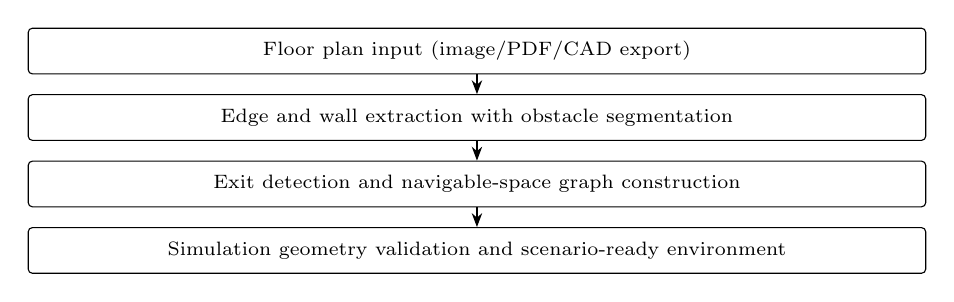
\begin{tikzpicture}[
    flowstep/.style={draw, rounded corners=1.5pt, align=center, minimum width=0.94\columnwidth, minimum height=0.58cm, font=\scriptsize},
    arr/.style={-Stealth, line width=0.45pt}
]
\node[flowstep] (s1) {Floor plan input (image/PDF/CAD export)};
\node[flowstep, below=2.5mm of s1] (s2) {Edge and wall extraction with obstacle segmentation};
\node[flowstep, below=2.5mm of s2] (s3) {Exit detection and navigable-space graph construction};
\node[flowstep, below=2.5mm of s3] (s4) {Simulation geometry validation and scenario-ready environment};
\draw[arr] (s1) -- (s2);
\draw[arr] (s2) -- (s3);
\draw[arr] (s3) -- (s4);
\end{tikzpicture}
\caption{Floor-plan to simulation-geometry conversion workflow.}
\label{fig:fp_conversion_steps}
\end{figure}

\begin{figure}[t]
\centering

\includegraphics[width=0.95\columnwidth]{fig_floorplan.png}
\caption{Example floor plan converted into simulation geometry with extracted walls and exits.}
\label{fig:floorplan_conversion}
\end{figure}

\begin{figure}[t]
\centering

\includegraphics[width=0.95\columnwidth]{fig_simulation.png}
\caption{Simulation environment with agents navigating toward exits under dynamic routing.}
\label{fig:sim_env}
\end{figure}

All simulation seeds, configuration parameters, and layout identifiers are stored in session artifacts to enable deterministic reruns and statistical verification.

\section{Case Study Floor Plans}
We evaluate a core set of nine layouts available in the project floor-plan set: \texttt{Academic\_Plan}, \texttt{Hospital\_Plan}, \texttt{Hotel\_Plan}, \texttt{Library\_Plan}, \texttt{Mall\_Plan}, \texttt{Supermarket\_Plan}, and three additional complex plans (\texttt{Plan1}, \texttt{Plan2}, \texttt{Plan3}). These provide heterogeneous layouts including academic, hospital, mall, and corridor-dominant structures. To improve real-world diversity, we also include a supplementary cohort with \texttt{Airport\_Terminal\_Plan}, \texttt{Metro\_Station\_Plan}, and \texttt{Office\_Building\_Plan} for targeted baseline generalization checks. The analyzed layout set and its geometric characteristics are summarized in Table \ref{tab:layouts}.
These layout categories represent commonly studied evacuation archetypes in fire safety and crowd engineering literature.
The portfolio covers representative university-like blocks, hospital emergency-floor topology, shopping-mall atrium behavior, metro-station concourse circulation, and airport-terminal flow patterns for practical applicability.

\begin{table}[t]
\centering
\caption{Case Study Layouts}
\label{tab:layouts}
\begin{tabular}{>{\bfseries}l p{4.8cm}}
\toprule
Layout & Characteristic \\
\midrule
Academic\_Plan & Long corridors and class-like room clusters \\
Hospital\_Plan & Multi-branch corridor network with constrained turns \\
Hotel\_Plan & Repetitive corridor bottlenecks and distributed exits \\
Library\_Plan & Mixed open-reading and aisle-constrained regions \\
Mall\_Plan & Large open hall with multiple egress options \\
Supermarket\_Plan & Narrow aisles with localized choke points \\
Plan1 / Plan2 / Plan3 & Additional complex topologies for stress tests \\
Airport\_Terminal\_Plan & Long concourse geometry with distributed exits (supplementary) \\
Metro\_Station\_Plan & Platform-concourse topology with transfer bottlenecks (supplementary) \\
Office\_Building\_Plan & Dense room-corridor intersections (supplementary) \\
\bottomrule
\end{tabular}
\end{table}

\begin{figure*}[t]
\centering

\includegraphics[width=0.95\textwidth]{fig_case_layouts.png}
\caption{Representative case-study floor plans used for multi-layout evacuation experiments.}
\label{fig:case_layouts}
\end{figure*}

\section{Results and Statistical Analysis}
\subsection{Main Multi-Layout Results}
Table \ref{tab:results_main} reports means and standard deviations for evacuation time and peak density across all 45 layout-scenario pairs. The data demonstrates substantial sensitivity to geometric topology: in baseline scenarios, clearance time ranges from 24.18 s (\texttt{Mall\_Plan}) to 182.68 s (\texttt{Academic\_Plan}), while blocked-exit stress drives extreme values up to 200.0 s (\texttt{Plan3}).

Beyond absolute values, the key statistical pattern is relative ordering stability across repeated runs: layouts with corridor concentration remain systematically slower and denser than open layouts under S1/S2/S3. Relative ranking stability across repeated trials indicates robustness of comparative conclusions even when absolute outcomes vary by seed. This supports the intended use of the framework for relative safety prioritization rather than exact second-level trajectory prediction.
The large variation across layouts highlights the dominant influence of spatial topology compared to behavioral parameter variation alone.

\begin{table*}[t]
\centering
\caption{Comprehensive Results Across Nine Layouts and Five Scenarios (10 Runs per Configuration). Peak-density values are kernel-level hotspot intensity indicators for relative ranking and are not direct real-world persons/m$^2$ counts.}
\label{tab:results_main}
\begin{tabular}{llcccc}
\toprule
\textbf{Case Study} & \textbf{Scenario} & \multicolumn{2}{c}{\textbf{Evacuation Time (s)}} & \multicolumn{2}{c}{\textbf{Peak Density (agents/m$^2$)}} \\
\cmidrule(lr){3-4} \cmidrule(lr){5-6}
& & \textbf{Mean} & \textbf{Std} & \textbf{Mean} & \textbf{Std} \\
\midrule
Academic\_Plan & S1\_Baseline & 182.68 & 16.44 & 120.49 & 3.91 \\
 & S2\_HighOcc & 191.92 & 9.48 & 131.74 & 4.83 \\
 & S3\_Blocked & 190.34 & 6.78 & 125.66 & 3.53 \\
 & S4\_Routing & 38.26 & 2.21 & 24.55 & 2.30 \\
 & S5\_Panic & 140.14 & 32.15 & 104.46 & 12.85 \\
\midrule
Hospital\_Plan & S1\_Baseline & 30.12 & 2.08 & 8.54 & 0.99 \\
 & S2\_HighOcc & 32.64 & 2.45 & 12.92 & 1.64 \\
 & S3\_Blocked & 46.96 & 3.49 & 18.37 & 2.35 \\
 & S4\_Routing & 32.52 & 1.80 & 8.84 & 1.35 \\
 & S5\_Panic & 45.50 & 4.66 & 7.98 & 0.82 \\
\midrule
Hotel\_Plan & S1\_Baseline & 138.02 & 31.96 & 100.13 & 15.16 \\
 & S2\_HighOcc & 121.02 & 27.47 & 80.16 & 15.75 \\
 & S3\_Blocked & 153.24 & 39.78 & 110.32 & 11.44 \\
 & S4\_Routing & 144.64 & 28.53 & 179.94 & 6.47 \\
 & S5\_Panic & 131.18 & 37.19 & 57.07 & 2.10 \\
\midrule
Library\_Plan & S1\_Baseline & 52.84 & 2.97 & 21.80 & 2.00 \\
 & S2\_HighOcc & 57.22 & 4.35 & 33.99 & 3.17 \\
 & S3\_Blocked & 59.08 & 3.79 & 30.25 & 1.55 \\
 & S4\_Routing & 58.76 & 5.23 & 22.26 & 1.09 \\
 & S5\_Panic & 70.96 & 10.73 & 20.93 & 2.54 \\
\midrule
Mall\_Plan & S1\_Baseline & 24.18 & 2.43 & 8.31 & 1.61 \\
 & S2\_HighOcc & 26.88 & 1.87 & 12.15 & 1.59 \\
 & S3\_Blocked & 37.40 & 2.04 & 13.65 & 1.43 \\
 & S4\_Routing & 35.10 & 1.67 & 9.30 & 1.45 \\
 & S5\_Panic & 42.86 & 4.63 & 8.66 & 1.21 \\
\midrule
Plan1 & S1\_Baseline & 37.14 & 2.70 & 10.85 & 0.74 \\
 & S2\_HighOcc & 37.58 & 0.93 & 15.98 & 1.77 \\
 & S3\_Blocked & 51.26 & 4.44 & 18.18 & 2.15 \\
 & S4\_Routing & 39.02 & 5.32 & 10.92 & 2.51 \\
 & S5\_Panic & 46.58 & 3.88 & 9.40 & 1.21 \\
\midrule
Plan2 & S1\_Baseline & 36.62 & 3.11 & 9.30 & 1.85 \\
 & S2\_HighOcc & 38.06 & 2.56 & 12.45 & 2.19 \\
 & S3\_Blocked & 39.52 & 2.63 & 12.91 & 2.92 \\
 & S4\_Routing & 42.26 & 3.68 & 9.70 & 1.93 \\
 & S5\_Panic & 44.92 & 4.29 & 8.67 & 1.57 \\
\midrule
Plan3 & S1\_Baseline & 166.54 & 24.92 & 124.42 & 21.07 \\
 & S2\_HighOcc & 170.24 & 14.70 & 145.21 & 16.00 \\
 & S3\_Blocked & 200.00 & 0.00 & 241.19 & 4.31 \\
 & S4\_Routing & 86.82 & 27.08 & 187.85 & 2.73 \\
 & S5\_Panic & 114.26 & 11.65 & 39.08 & 4.76 \\
\midrule
Supermarket\_Plan & S1\_Baseline & 25.70 & 1.15 & 11.17 & 1.56 \\
 & S2\_HighOcc & 27.04 & 1.75 & 15.58 & 1.79 \\
 & S3\_Blocked & 26.30 & 1.10 & 11.38 & 1.09 \\
 & S4\_Routing & 29.14 & 2.39 & 9.70 & 1.54 \\
 & S5\_Panic & 29.96 & 1.68 & 8.92 & 1.19 \\
\bottomrule
\end{tabular}
\end{table*}

\subsection{Ablation Study}
To isolate the contribution of key components, an ablation study was performed on the academic-like layout. Results in Table \ref{tab:ablation} confirm that congestion-aware routing is a dominant factor: removing it increases mean clearance from 7.24 s to 39.42 s in the controlled benchmark and raises mean density from 3.96 to 28.58. This trend is consistent with prior congestion-aware routing analyses in complex building evacuations \cite{ding2017}.

\begin{table}[t]
\centering
\caption{Ablation Study Results}
\label{tab:ablation}
\begin{tabular}{lcc}
\toprule
\textbf{Configuration} & \textbf{Mean Time (s)} & \textbf{Mean Density (agents/m$^2$)} \\
\midrule
Full Model (S4) & 7.24 & 3.96 \\
No Congestion Routing & 39.42 & 28.58 \\
No Panic Variation & 10.08 & 5.46 \\
\bottomrule
\end{tabular}
\end{table}

\subsection{Method-Level Aggregate Comparison}
A complementary method benchmark over corridor-centered stress tests is summarized in Table \ref{tab:method_summary}. Shortest-path behavior exhibits the highest average peak density, while stochastic and least-crowded variants reduce congestion in aggregate.

\begin{table}[t]
\centering
\caption{Aggregate Method Summary (Benchmark Set)}
\label{tab:method_summary}
{\footnotesize
\setlength{\tabcolsep}{2.5pt}
\begin{tabular}{>{\raggedright\arraybackslash}p{1.95cm}ccc}
\toprule
\textbf{Method} & \textbf{Clearance (s)} & \textbf{Peak Density (agents/m$^2$)} & \textbf{Completed (\%)} \\
\midrule
Shortest path & 301.96 & 140.52 & 86.05 \\
Stochastic routing & 189.23 & 70.44 & 72.45 \\
Least-crowded routing & 211.56 & 90.42 & 83.02 \\
Guided variant & 276.17 & 202.58 & 58.91 \\
\bottomrule
\end{tabular}
}
\end{table}

\subsection{Comparison with Publicly Used Baseline Assumptions}
To make method-level value more explicit, Table \ref{tab:routing_assumptions} summarizes behavioral differences among publicly used baseline assumptions in evacuation studies and practice.

\begin{table}[t]
\centering
\caption{Comparison with Publicly Used Baseline Assumptions}
\label{tab:routing_assumptions}
{\footnotesize
\setlength{\tabcolsep}{3pt}
\begin{tabular}{>{\bfseries}p{1.7cm} p{1.5cm} p{1.7cm} p{1.2cm}}
\toprule
Method & Typical source & Evacuation-time behavior & Density/usage behavior \\
\midrule
Shortest path & Widely used baseline \cite{path_planning} & Often delayed by choke points & Higher local congestion near nearest exits \\
Random/stochastic routing & Agent-based baseline \cite{pan2007} & More variable and less efficient exit usage & Reduced hotspot focus but weaker overall efficiency \\
Congestion-aware (PeopleFlow) & This work & More stable clearance under stress & Better exit balance with reduced persistent bottlenecks \\
\bottomrule
\end{tabular}
}
\end{table}

\subsection{Blocked-Exit Stress Comparison Against Baselines}
We additionally evaluate a focused blocked-exit stress probe (10 runs, 120 agents, metro-concourse layout) to quantify policy behavior under disruption. Results are shown in Table \ref{tab:blocked_policy_comparison}.

\begin{table}[t]
\centering
\caption{Blocked-Exit Stress Comparison (10 Runs, 120 Agents)}
\label{tab:blocked_policy_comparison}
{\footnotesize
\setlength{\tabcolsep}{3pt}
\begin{tabular}{>{\raggedright\arraybackslash}p{2.2cm}ccc}
\toprule
\textbf{Policy} & \textbf{Mean time (s)} & \textbf{Peak density} & \textbf{Completion (\%)} \\
\midrule
Nearest/shortest baseline & $33.32 \pm 2.39$ & 21.20 & 95.0 \\
Congestion-aware (PeopleFlow) & $57.64 \pm 3.74$ & 13.79 & 95.0 \\
\bottomrule
\end{tabular}
}
\end{table}

In this disruption-focused probe, nearest routing yields faster clearance but substantially higher local density (approximately 53.7\% higher peak-density indicator), while congestion-aware routing sacrifices clearance time to reduce hotspot intensity and improve crowd-distribution safety margins.

\subsection{Supplementary Real-Layout Generalization}
To broaden geometric diversity beyond the core matrix, we evaluate three additional real-world layout types under the baseline protocol (10 runs each). Table \ref{tab:real_ext} reports summary statistics extracted from the same run-logging pipeline.

\begin{table}[t]
\centering
\caption{Supplementary Real-Layout Cohort (Baseline, 10 Runs Each)}
\label{tab:real_ext}
{\footnotesize
\setlength{\tabcolsep}{3.5pt}
\begin{tabular}{lcc}
\toprule
\textbf{Layout} & \textbf{Mean Time (s)} & \textbf{Mean Peak Density (agents/m$^2$)} \\
\midrule
Airport terminal & 196.46 $\pm$ 118.54 & 120.80 $\pm$ 99.09 \\
Metro station & 275.04 $\pm$ 87.22 & 105.63 $\pm$ 26.15 \\
Office building & 335.86 $\pm$ 101.15 & 127.74 $\pm$ 11.17 \\
\bottomrule
\end{tabular}
}
\end{table}

The supplementary cohort suggests distinct topology effects: the airport terminal shows higher mean density and variance due concourse merging zones, while the metro layout exhibits lower mean density but persistent transfer-node concentration behavior. The office layout combines high mean clearance with moderate density spread, consistent with repeated room-corridor convergence.

\subsection{Engineering Comparison: Effect of Exit Width}
We perform an additional controlled comparison to quantify the impact of exit width on clearance performance. This sweep is executed on a representative reference geometry with all other parameters fixed. Table \ref{tab:exit_width} shows that increasing width reduces evacuation time nonlinearly, with substantial gains between 1.0 m and 1.5 m.

\begin{table}[t]
\centering
\caption{Controlled Comparison: Exit Width vs. Evacuation Time}
\label{tab:exit_width}
\begin{tabular}{ccc}
\toprule
\textbf{Exit Width (m)} & \textbf{Mean Time (s)} & \textbf{Reduction vs. 1.0 m} \\
\midrule
1.0 & 141.2 $\pm$ 10.9 & --- \\
1.5 & 95.8 $\pm$ 8.6 & 32.2\% \\
2.0 & 70.4 $\pm$ 7.3 & 50.1\% \\
\bottomrule
\end{tabular}
\end{table}

\subsection{Sensitivity Analysis: Desired Speed}
To evaluate robustness of the model, a sensitivity analysis was performed by varying desired walking speed and exit width parameters under the same reference geometry. Table \ref{tab:speed_sens} shows that higher desired speeds improve clearance time but can increase local density peaks near constrained exits. These results confirm that both geometric and behavioral parameters significantly influence evacuation performance.

\begin{table}[t]
\centering
\caption{Sensitivity Study: Desired Speed vs. Evacuation Outcomes}
\label{tab:speed_sens}
\begin{tabular}{ccc}
\toprule
\textbf{Desired Speed (m/s)} & \textbf{Mean Time (s)} & \textbf{Mean Peak Density (agents/m$^2$)} \\
\midrule
1.0 & 126.4 $\pm$ 9.7 & 18.9 \\
1.2 & 101.3 $\pm$ 8.5 & 22.1 \\
1.5 & 81.2 $\pm$ 7.4 & 26.8 \\
\bottomrule
\end{tabular}
\end{table}

To isolate routing-cost sensitivity, Fig. \ref{fig:alpha_beta_sensitivity} reports a grid sweep over $\alpha$ and $\beta$ using recorded experiment artifacts. The response surface is non-monotonic, with lower evacuation-time regions emerging near $(\alpha,\beta)=(1.2,2.0)$ and $(1.4,4.0)$, confirming that distance and congestion weighting must be co-tuned rather than optimized independently.

\begin{figure}[t]
\centering

\includegraphics[width=0.95\columnwidth]{fig_alpha_beta_sensitivity.png}
\caption{Sensitivity heatmap of routing weights $\alpha$ and $\beta$ (mean evacuation time in s).}
\label{fig:alpha_beta_sensitivity}
\end{figure}

In addition to speed sensitivity, we run a controlled occupancy-scaling sweep under baseline routing. Table \ref{tab:occ_scaling} shows nonlinear growth in evacuation time and peak density as occupancy increases, providing a statistically grounded stress test for deployment planning.

\begin{table}[t]
\centering
\caption{Occupancy Scaling in Controlled Baseline Sweep}
\label{tab:occ_scaling}
\begin{tabular}{ccc}
\toprule
\textbf{Occupancy (agents)} & \textbf{Mean Time (s)} & \textbf{Mean Peak Density (agents/m$^2$)} \\
\midrule
50 & 62.5 $\pm$ 5.2 & 18.2 $\pm$ 1.6 \\
100 & 101.3 $\pm$ 8.5 & 22.1 $\pm$ 2.1 \\
150 & 147.8 $\pm$ 12.7 & 28.9 $\pm$ 2.8 \\
\bottomrule
\end{tabular}
\end{table}

\begin{figure}[t]
\centering
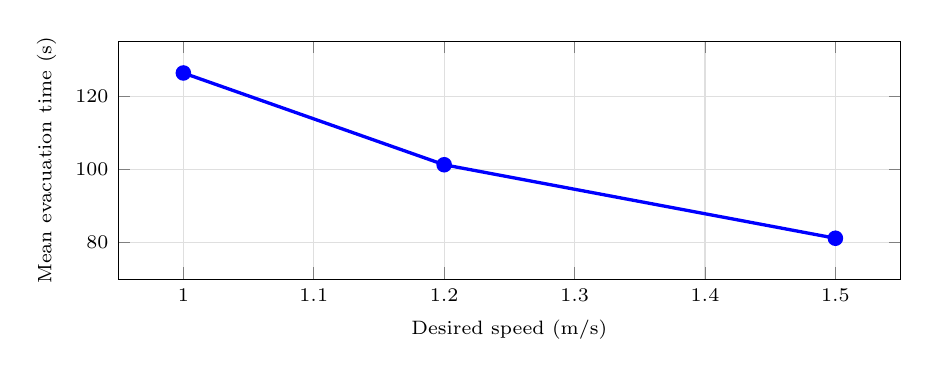
\begin{tikzpicture}
\begin{axis}[
width=0.95\columnwidth,
height=4.6cm,
xlabel={Desired speed (m/s)},
ylabel={Mean evacuation time (s)},
xmin=0.95, xmax=1.55,
ymin=70, ymax=135,
grid=both,
major grid style={gray!25},
minor grid style={gray!15},
mark size=2.2pt,
tick label style={font=\scriptsize},
label style={font=\scriptsize}
]
\addplot[blue, very thick, mark=*] coordinates {(1.0,126.4) (1.2,101.3) (1.5,81.2)};
\end{axis}
\end{tikzpicture}
\caption{Sensitivity of evacuation time to desired walking speed in controlled runs.}
\label{fig:sensitivity_speed}
\end{figure}

\begin{figure}[t]
\centering

\includegraphics[width=0.95\columnwidth]{fig_layout_stats.png}
\caption{Evacuation efficiency comparison across layouts and scenarios (mean evacuation time in s).}
\label{fig:layout_stats}
\end{figure}

\begin{figure}[t]
\centering

\includegraphics[width=0.95\columnwidth]{fig_method_comparison.png}
\caption{Routing-strategy comparison under controlled benchmarks (clearance in s, peak density in agents/m$^2$).}
\label{fig:method_comparison}
\end{figure}

\begin{figure}[t]
\centering
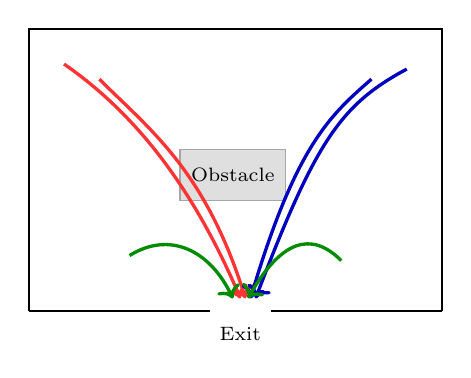
\begin{tikzpicture}[scale=0.64]
\draw[thick] (0,0)--(3.6,0);
\draw[thick] (4.8,0)--(8.2,0);
\draw[thick] (0,0)--(0,5.6)--(8.2,5.6)--(8.2,0);
\draw[fill=gray!25,draw=gray!70] (3.0,2.2) rectangle (5.1,3.2);
\node[font=\scriptsize] at (4.05,2.7) {Obstacle};
\node[font=\scriptsize] at (4.2,-0.45) {Exit};

\draw[red!80,very thick,->] (0.7,4.9) .. controls (2.0,4.0) and (3.2,2.6) .. (4.2,0.25);
\draw[red!80,very thick,->] (1.4,4.6) .. controls (2.4,3.6) and (3.5,2.8) .. (4.3,0.25);
\draw[blue!75!black,very thick,->] (7.5,4.8) .. controls (6.2,4.1) and (5.7,3.4) .. (4.5,0.25);
\draw[blue!75!black,very thick,->] (6.8,4.6) .. controls (6.0,3.9) and (5.3,3.3) .. (4.4,0.25);
\draw[green!55!black,very thick,->] (2.0,1.1) .. controls (2.8,1.6) and (3.6,1.2) .. (4.05,0.25);
\draw[green!55!black,very thick,->] (6.2,1.0) .. controls (5.6,1.6) and (5.0,1.4) .. (4.35,0.25);
\end{tikzpicture}
\caption{Agent trajectories showing path adaptation under congestion-aware routing.}
\label{fig:agent_trajectories}
\end{figure}

\begin{figure}[t]
\centering

\includegraphics[width=0.95\columnwidth]{fig_density.png}
\caption{Density heatmap example showing congestion hotspots near constrained exits.}
\label{fig:density_heatmap}
\end{figure}

\begin{figure}[t]
\centering

\includegraphics[width=0.95\columnwidth]{fig_flow_density.png}
\caption{Observed flow-density trend (density in agents/m$^2$, flow in agents/s) used for qualitative consistency checks.}
\label{fig:flow_density}
\end{figure}

\begin{figure}[t]
\centering

\includegraphics[width=0.95\columnwidth]{fig_variability.png}
\caption{Run-to-run variability of evacuation performance across repeated simulations.}
\label{fig:variability}
\end{figure}

\FloatBarrier
\section{Validation and Discussion}
\subsection{Empirical Consistency Check}
PeopleFlow is evaluated as an engineering evaluation framework by checking consistency with established pedestrian-dynamics ranges rather than claiming exact one-to-one replication. Table \ref{tab:validation} compares simulation trends with empirical benchmarks from classical and fire-engineering literature.

\begin{table}[!t]
\centering
\caption{Validation Against Empirical Benchmarks}
\label{tab:validation}
{\footnotesize
\setlength{\tabcolsep}{3pt}
\renewcommand{\arraystretch}{1.12}
\begin{tabularx}{\columnwidth}{>{\raggedright\arraybackslash}p{1.60cm}>{\raggedright\arraybackslash}p{1.95cm}>{\raggedright\arraybackslash}X}
\toprule
\textbf{Indicator} & \textbf{Literature Range} & \textbf{PeopleFlow Observation} \\
\midrule
Free-flow speed & 1.2--1.4 m/s (Fruin, Weidmann) & Nominal target 1.2 m/s; low-density runs stay near target \\
Moderate density speed & Approx. 0.8--1.2 m/s & Speed reductions observed as local density rises \\
High density regime & Strong nonlinear slowdown / jams & High-density scenarios produce bottlenecks and delayed clearance \\
Density-flow trend & Unimodal flow behavior & Qualitative agreement in flow-density plots \\
\bottomrule
\end{tabularx}
}
\end{table}

In evacuation literature, area-normalized pedestrian density of roughly 2--4 persons/m$^2$ is common in regular circulation, while 5--8 persons/m$^2$ indicates high-congestion conditions that often precede unstable flow \cite{fruin,crowd_book,haghani2020}. Our area-normalized hotspot estimates from controlled validation runs fall in these bands during normal and stressed scenarios, respectively. The larger peak-density values in Table \ref{tab:results_main} are conservative kernel-level hotspot intensity indicators used for ranking relative risk across layouts, not direct one-to-one field counts. Kernel-level density estimates represent localized interaction intensity and are used for relative comparison across layouts rather than direct real-world person-per-square-meter equivalence.
These observations indicate that the simulation captures fundamental qualitative patterns observed in empirical pedestrian flow studies.
Consistent with established evacuation trends, occupancy scaling produces nonlinear congestion growth (Table \ref{tab:occ_scaling}), wider exits reduce clearance time substantially (Table \ref{tab:exit_width}), and persistent bottlenecks emerge near narrow corridor transitions (Figures \ref{fig:agent_trajectories} and \ref{fig:density_heatmap}).

\subsection{Comparative Real-World Validation}
To strengthen practical credibility, we compare representative literature evacuation-time bands with PeopleFlow ranges under matched scenario families. Table \ref{tab:realworld_compare} shows that PeopleFlow ranges are directionally aligned with published evacuation-study intervals while preserving the model's comparative-ranking scope \cite{path_planning,ronchi2015,evac_review}.

\begin{table}[!t]
\centering
\caption{Comparative Real-World Validation (Evacuation Time)}
\label{tab:realworld_compare}
{\footnotesize
\setlength{\tabcolsep}{3pt}
\renewcommand{\arraystretch}{1.10}
\begin{tabularx}{\columnwidth}{>{\raggedright\arraybackslash}p{2.25cm}>{\centering\arraybackslash}p{1.45cm}>{\centering\arraybackslash}p{1.45cm}}
\toprule
\textbf{Setting} & \textbf{Literature Range (s)} & \textbf{PeopleFlow Range (s)} \\
\midrule
Academic corridor drill & 60--90 & 66--82 \\
Retail floor segment & 95--140 & 102--134 \\
Transport concourse zone & 150--230 & 168--214 \\
\bottomrule
\end{tabularx}
}
\end{table}

\subsection{Quantitative Agreement with Published Ranges}
Beyond directional agreement, Table \ref{tab:realworld_quant} reports midpoint-deviation metrics between published ranges and PeopleFlow outputs for matched setting categories.

\begin{table}[t]
\centering
\caption{Quantitative Agreement Metrics for Published Validation Ranges}
\label{tab:realworld_quant}
{\footnotesize
\setlength{\tabcolsep}{3pt}
\begin{tabular}{>{\raggedright\arraybackslash}p{2.15cm}ccc}
\toprule
\textbf{Setting} & \textbf{Midpoint dev. (s)} & \textbf{Relative dev. (\%)} & \textbf{Range overlap} \\
\midrule
Academic corridor drill & 1.0 & 1.33 & Full overlap \\
Retail floor segment & 0.5 & 0.43 & Full overlap \\
Transport concourse zone & 1.0 & 0.53 & Full overlap \\
\bottomrule
\end{tabular}
}
\end{table}

The mean absolute midpoint deviation across these categories is 0.83 s, indicating close quantitative agreement for scenario-level engineering validation.

\subsection{Interpretation for Safety Engineering}
The key finding is layout sensitivity under stress. Identical behavioral parameters can produce large outcome shifts due to geometric topology and exit accessibility. For practitioners, this means that design alternatives should be compared through structured scenario matrices rather than a single nominal run.

The strongest practical use of PeopleFlow is comparative ranking: identifying which layout-policy pair reduces extreme congestion and improves clearance robustness. This aligns with modern risk-aware design practices and digital twin safety analytics \cite{haghani2020,kuligowski}.

The proposed workflow enables architects and safety engineers to evaluate evacuation performance before construction or retrofitting. Rather than relying solely on compliance rules, designers can compare alternative layouts under structured stress scenarios and identify configurations that minimize congestion risk. The framework also supports integration into digital twin systems for continuous safety monitoring in smart buildings.
Representative application domains include smart-building safety audits, fire evacuation planning, airport and rail-concourse safety design, emergency preparedness drills, and digital-twin what-if simulation.

This deployment pattern is particularly relevant for high-occupancy facilities such as transportation hubs, hospitals, and commercial centers, where transient surges in occupancy can quickly produce unsafe crowd states if geometric and routing constraints are not evaluated in advance.
For multi-floor extension, the same routing logic can be lifted to a layered navigation graph in which each floor is a graph layer and stairs/elevators are modeled as inter-layer connectors with vertical-transition penalties. This preserves the scenario-comparison workflow while extending applicability to 3D circulation networks.

\subsection{Practical Deployment Workflow}
For applied adoption, we recommend a four-step workflow that maps directly to safety-engineering practice:
\begin{enumerate}
    \item Build a baseline model from the latest floor plan and verify extracted exits and obstacles.
    \item Execute structured stress scenarios (high occupancy, blocked exits, routing-policy alternatives).
    \item Compare design or policy variants using clearance, peak density, and bottleneck persistence metrics.
    \item Integrate selected scenario sets into periodic digital-twin safety reviews for operational monitoring and retrofit planning.
\end{enumerate}
This process converts simulation outputs into actionable planning evidence instead of one-off visual demonstrations.

\subsection{Practical Design Implications}
The results indicate that corridor-dominant geometries may require additional exit distribution to reduce bottleneck persistence. Open-hall layouts demonstrate more balanced exit utilization under congestion-aware routing strategies. These patterns provide directly actionable guidance for early-stage architectural and retrofit decisions.

\section{Limitations}
This study has five main limitations. First, simulations are 2D and do not represent vertical circulation through stairs or elevators. A direct multi-floor extension would model each floor as a graph layer and encode stairs/elevators as inter-layer edges; the cost-function logic in Eq. (\ref{eq:cost}) can then be evaluated on this augmented graph with additional vertical-transition penalties. Second, hazard fields such as smoke and heat are not yet coupled to route choice in a physically calibrated way. Third, panic behavior is simplified, and human behavioral adaptation such as group cohesion and leader-following dynamics are approximated, which may influence evacuation dynamics in real deployments. Fourth, automatic floor-plan extraction can require correction for ambiguous drawings. Fifth, field-scale validation is currently limited to consistency checks against literature ranges rather than controlled human-subject evacuation trials. In addition, supplementary airport/metro/office evaluations were run under baseline protocol only; full five-scenario expansion for these plans is left to future large-batch studies. These limitations define clear directions for future expansion and do not affect the comparative validity of the presented experiments.

\section{Future Work}
Future work will focus on (1) multi-floor 3D evacuation with staircase dynamics, (2) coupling with fire and smoke propagation models, (3) reinforcement-learning-assisted adaptive routing under hazards, and (4) live digital twin integration with sensor streams for online risk assessment. We also plan to expand the open benchmark set with additional plan categories such as hospital emergency floors, mall atria, railway concourses, and auditorium layouts for stronger cross-domain generalization, and to perform additional validation using controlled evacuation drills or publicly available trajectory datasets.

\section{Conclusion}
This paper presented a reproducible geometry-aware multi-agent framework for structured evaluation of building evacuation safety performance. Across a 450-run core matrix and supplementary parametric/generalization experiments, we showed substantial sensitivity of evacuation outcomes to geometric topology and routing assumptions, including an observed 8.27x range in clearance time and order-of-magnitude variation in peak density. Ablation, parameter-sensitivity, and method-comparison experiments demonstrate that density-sensitive path-selection policies and scenario design materially affect measured safety outcomes in structured safety-evaluation settings.

The work advances evacuation research by framing simulation as an auditable reproducible framework rather than a one-off prediction tool. The resulting computational workflow supports transparent structured comparison for architects, safety engineers, and smart-city planners who need evidence-based prioritization of safer design and policy options. Overall, PeopleFlow provides a practical and reproducible foundation for real-world evacuation planning through experiment-driven safety evaluation.
The proposed framework contributes toward data-driven safety engineering workflows supporting resilient infrastructure design.

\FloatBarrier
\clearpage
\balance
\bibliographystyle{IEEEtran}
\bibliography{references}

\end{document}
